\section{MPI}
Initially a rudimentary analysis of the serial code was conducted to analyse the complexity. The main bottleneck comes
from the double for loop in the compute\_time\_step function which has a complexity of $\mathcal{O}(nx*ny)$. This function
then gets called $\frac{Tend}{dt}$ times. So the complexity is $\mathcal{O}(nx*ny*Tend/dt)$. Taking this a bit further
we can make the simplification that $dt \propto \frac{1}{nx}$, so we can say that the complexity is roughly
$\mathcal{O}(nx^2*ny)$. Next we needed to profile the code to figure out the portion of the code that could be
parallelized. This was performed using the perf tool in Linux. This analysis revealed at the solve function was taking
up 92.61\% of the code time, and since the entirety of the solve function can be parallelized this was taken to be the
fraction of parallelizable code. Conversely, 7.29\% was taken to be the fraction of serial code. Calculate the
theoretical strong and weak scaling laws:

\begin{figure}[h!]
    \centering
    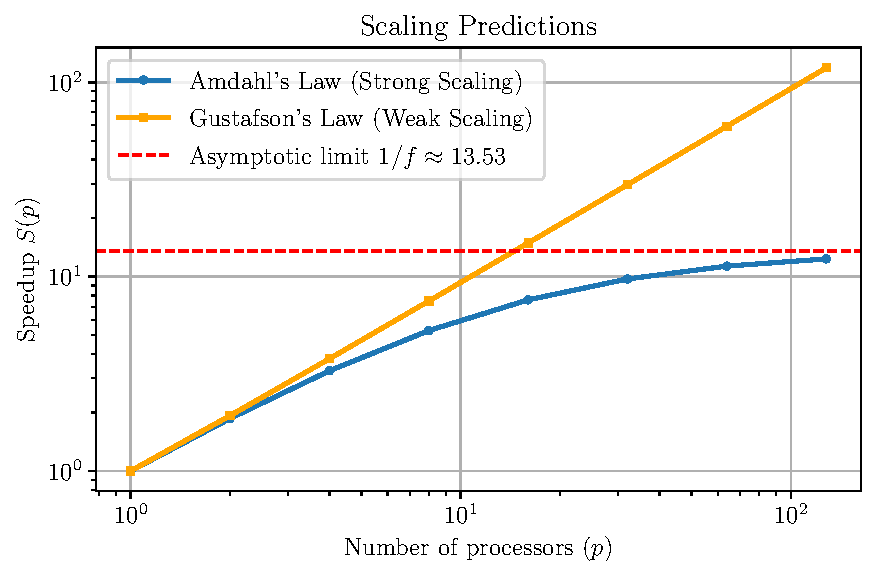
\includegraphics[width=0.7\textwidth]{./plots/scaling_laws.pdf}\\[1cm]
    \caption{Amdahl's Law (Strong Scaling) and Gustafson's Law (Weak Scaling)}
\end{figure}
\FloatBarrier

To parallelize the code I opted for a 2D domain decomposition as well as a Cartesian communicator structure to allow for
easy communication with the neighbours. Each local section of the domain also needed to have a halo region which would
mirror the values of its neighbouring region. At each iteration we ``exchange'' these halo regions with the neighbours.
In this way each processor can work on their local domain and will only need to communicate to access the relevant parts
from its neighbours. Shown in the graphs below are the results from the strong and weak scaling experiments with the MPI
code.
\begin{figure}[h!]
    \begin{subfigure}{0.5\textwidth}
        \centering
        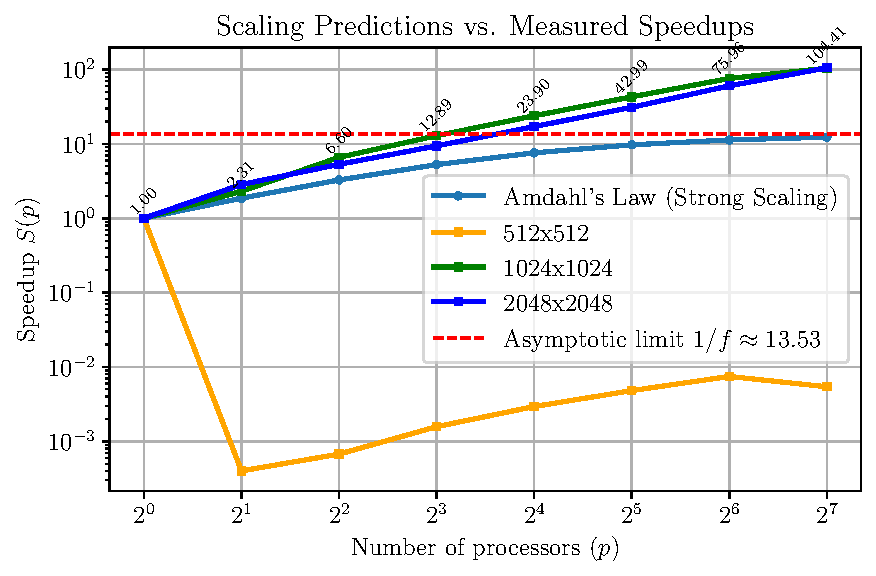
\includegraphics[width=0.95\linewidth]{./plots/strong_scaling.pdf}
        \caption{Observed Strong Scaling for various problem sizes}
        \label{fig:strong_scaling}
    \end{subfigure}
    \hfill
    \begin{subfigure}{0.5\textwidth}
        \centering    
        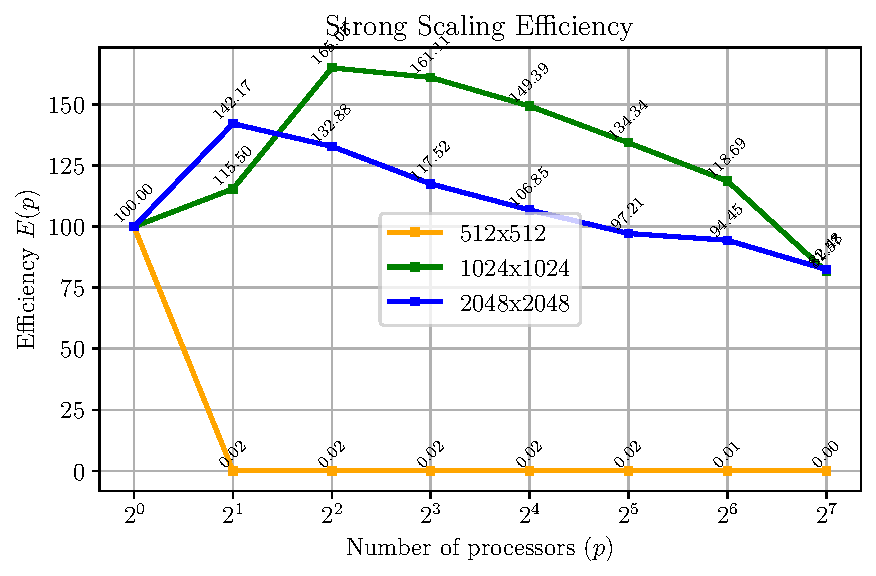
\includegraphics[width=0.95\linewidth]{./plots/strong_scaling_efficiency.pdf}
        \caption{Observed Strong Scaling Efficiency for various problem sizes}
        \label{fig:strong_scaling_efficiency}
    \end{subfigure}
\end{figure}

\begin{figure}[h!]
    \begin{subfigure}{0.5\textwidth}
        \centering
        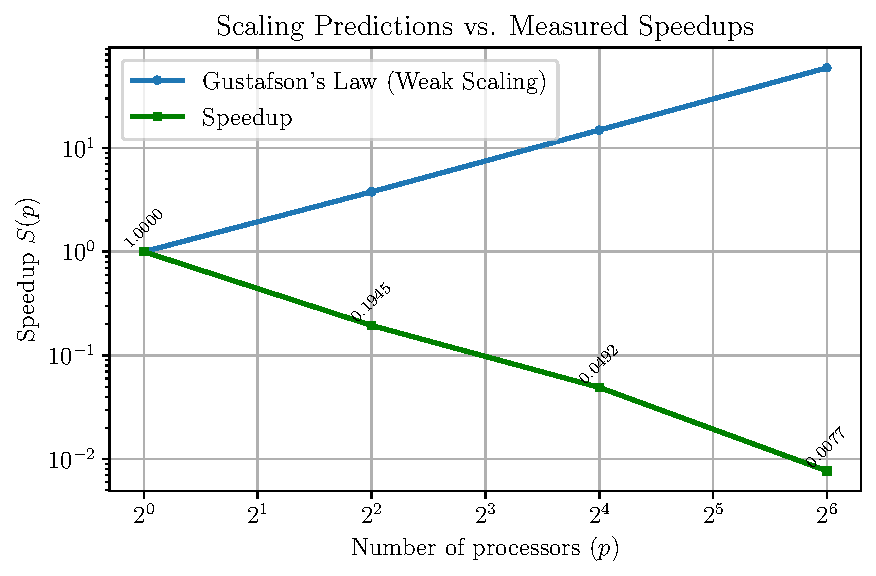
\includegraphics[width=0.95\linewidth]{./plots/weak_scaling.pdf}
        \caption{Observed Weak Scaling for various problem sizes}
    \end{subfigure}
    \hfill
    \begin{subfigure}{0.5\textwidth}
        \centering
        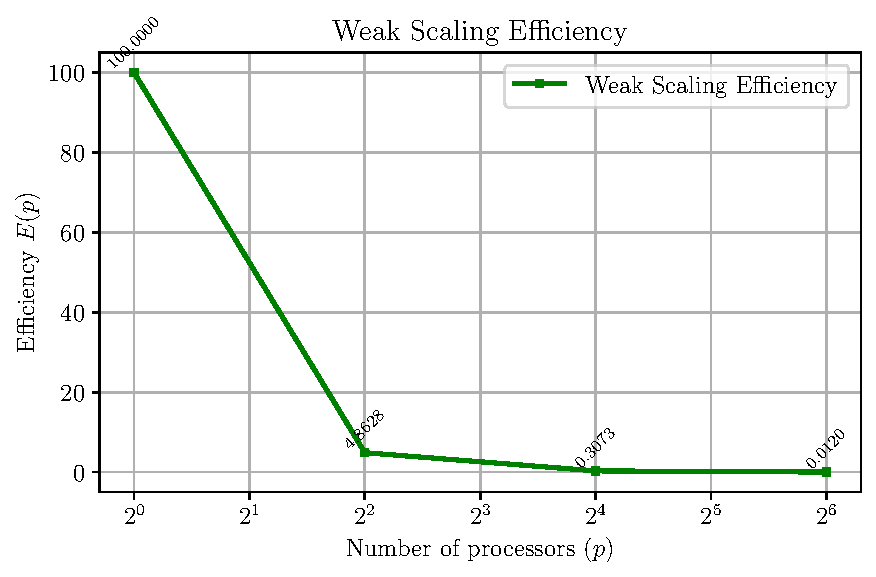
\includegraphics[width=0.95\linewidth]{./plots/weak_scaling_efficiency.pdf}
        \caption{Observed Weak Scaling Efficiency for various problem sizes}
    \end{subfigure}
    \label{fig:weak_scaling}
\end{figure}

\FloatBarrier
For the weak scaling experiments, the domain size was quadruped along with the processor count starting with a domain
size of 32x32 and a processor count of 1. There are two main things we can notice from \autoref{fig:strong_scaling}. One, our estimate of $\alpha$, was not
correct as empirically we see speed-ups above Amdahl's law. This can be fixed with a higher sampling rate in perf,
however the file sizes generated by perf at the higher sampling rates often passed 100GB and so could not be stored on
my home partition. At a rough glance, I estimate that the proportion of code that could be parallelized is closer to
$98-99\%$. Secondly, we see that MPI parallelism only makes sense for large domain sizes. If the domain size is too
small (as is the 512x512 case), the overhead of communication becomes larger than the potential speed-ups from
parallelism. When looking at \autoref{fig:strong_scaling_efficiency}, we can see that there is a peak efficiency for a
problem size that is big enough to be worth parallelizing. Past this peak, adding more processors may provide an
additional speed-up however, the effect may not be as noticeable. When looking at \autoref{fig:weak_scaling}, we see
that the MPI code scales quite poorly as the problem size increases, indicating that perhaps the communication cost in
the code does not scale linearly, and at the higher processor counts there is a lot of communication involved.


